\documentclass[oneside,a4paper,english,links]{article}
%
\usepackage{graphicx}
\usepackage{amsmath,amsfonts}
\usepackage{url}
\usepackage{subfig}
\usepackage{ amssymb }

\newcommand{\rodrigo}[1]{\authnote{Rodrigo}{#1}}

\title{Fractal and Multifractal analysis of images}

\author{Rodrigo Baravalle}

\begin{document}

\maketitle
\begin{center}
\small{Laboratorio de Sistemas Din\'amicos y Procesamiento de Informaci\'on, FCEIA, Universidad Nacional de Rosario - CIFASIS - CONICET}\\
\small{Riobamba 250 bis, 2000, Rosario, Argentina}\\

\texttt{baravalle@cifasis-conicet.gov.ar}\\
\texttt{\url{http://www.cifasis-conicet.gov.ar/index.php?grupo=4}}
\end{center}

\begin{abstract}
In the last years, fractals and multifractals have been used extensively in image processing. They have shown to provide local and global image features that are both robust and low dimensional.

Adequate image descriptors are fundamental in image classification, object recognition and characterization. Main requirements for image features are robustness and low dimensionality.

In this work several fractal and multifractal techniques for image analysis are presented.
\end{abstract}

\section{Introduction}
A great number of physical systems tend to present similar behaviours on different scales of observation. In the last century, the mathematician Mandelbrot employed the term {\em fractal} to describe objects whose complex geometry cannot be characterized by an integral dimension. In other words, Euclidean geometry fails to successfully describe those systems.

Fractal and multifractal analysis of images have proved to capture useful properties of the underlying material being represented. Characterisation of images using these features have been successfully applied in different areas, such as medicine \cite{Andjelkovic2008,Yu2011} and texture classification \cite{Wendt2009}. Through several procedures, it is possible to obtain different Fractal Dimensions (FD), each of them capturing a different property of the material ({\em e.g.}, void image fraction, rugosity).

In this work we will show different fractal and multifractal dimensions employed in different applications such as classification and edge detection. In section 2 we briefly introduce the theory underlying fractal sets. In section 3 we describe an example of the materials and methods employed in a classification. In section 4 we show the results obtained in that classification. In section 5 we show different possible applications of fractal and multifractal analysis. In section 6 we summarise the conclusions.

\section{Fractal analysis}
\subsection{Fractal}
An useful property to understand fractals is its autosimilarity, {\em i.e.}, the entire structure is contained as a substructure. Since in nature it is not always the case, usually fractals are characterized by statistical self-similarity. Examples of natural fractals are trees, clouds, mountains, coastlines and even heartbeats. In Figure \ref{fig:fractal} an image of showing statistical self-similarity is shown.

\begin{figure*}[htb]
\centering
$\vcenter{\hbox{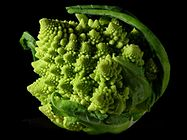
\includegraphics[scale=1.3]{imagenes/fractal}}}$
\caption{An image of a Romanesco Broccoli showing statistical self-similarity}
\label{fig:fractal}
\end{figure*}


An image representing an object could be processed in order to obtain its fractal dimensions, using the algorithms presented in next sections.

\subsection{Box dimension}
Box FD is a simplification of the Hausdorff (originally Minkowski - Bouligand) dimension for non strictly self-similar objects (\cite{Peitgen2004}). Given a binarised image, it is subdivided in a grid of size $M\times M$ where the side of each box formed is $\epsilon$. If $N_{\epsilon}$ represents the amount of boxes that contains at least one pixel in the binarisation of the set for that $\epsilon$, then the box dimension  $D_{b}$ is defined as

\begin{equation}
D_{b} \triangleq \displaystyle\lim_{\epsilon \to 0}{\frac{\log(N_{\epsilon})}{\log (1/\epsilon)}}.
\label{eqn:eqn1}
\end{equation}

The algorithm computes a binarised image from the original one and then selects different values of $\epsilon$ in it, making a count of the boxes that contains pixels in each case (to avoid numerical instabilities, a mean of cases is computed, establishing different positions in the grid over the image). Finally, a linear regression adjustment is made with the obtained data, in the $\log-\log$ space, and the slope of the straight line is by definition the box dimension of the image. In Fig. \ref{fig:fitbox} an image of the bread type {\em salvado} is shown with its corresponding box dimension computation.

\begin{figure*}[htb]
\centering
$\vcenter{\hbox{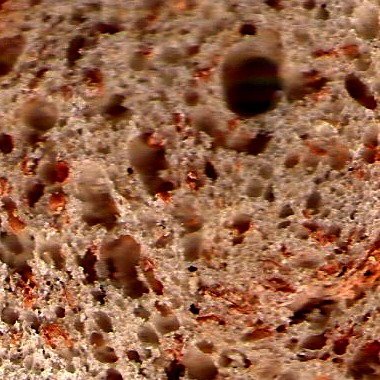
\includegraphics[scale=1.3]{imagenes/salvado19}}}$
$\vcenter{\hbox{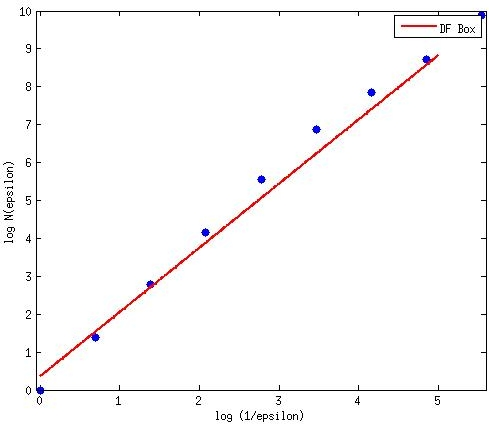
\includegraphics[scale = 0.4]{imagenes/fitbox}}}$
\caption{An image and its computed box dimension}
\label{fig:fitbox}
\end{figure*}

\subsection{Morphological fractal}
This FD is computed through dilation and erosion operations, using a structuring element (SE). The transformed image is a function of the distribution of that particular SE in the original image.  In \cite{Gonzales2008}, the SE selected was a rhombus $Y$ with scales that varies from $\epsilon = 1$ to $\epsilon = 7$ (and the areas of the SE between $5$ and $113$ pixels). The surface area $S(X,Y,\epsilon)$ can be calculated, for each $\epsilon$ as

\begin{equation}
S(X,Y,\epsilon) = \frac{\sum_{x,y \in M} (f_{\epsilon}^{u}(x,y) - f_{\epsilon}^{l}(x,y))}{2\epsilon},
\label{eqn:eqn2}
\end{equation}
\noindent
where $f_{\epsilon}^{u}(x,y)$ is the $\epsilon$-th dilation and $f_{\epsilon}^{l}(x,y)$ is the $\epsilon$-th erosion of the original image. The morphological FD $M_{d}$ is estimated from the slope of a linear regression adjustment of the data in $S(X,Y,\epsilon)$ and $\epsilon$ in the $\log-\log$ space as

\begin{equation}
M_{d} = 2 + m,
\label{eqn:eqn3}
\end{equation}
\noindent
where $m$ is the slope of the straight line fit.

\section{Multifractal analysis}
The fractal dimension is an exponent which relates the statistical self-similarity of the object at different scales. On the one hand, deterministic fractals are characterized by one FD. They are called {\em monofractals} (for instance, Koch Curve, Sierpinsky triangle). On the other hand, {\em multifractals} (\cite{Mandelbrot89}) are characterized by a set of FDs. It is assumed that these structures are composed by different fractals coexisting simultaneously.

\subsubsection{H\"older exponent}
Informally, the way to proceed with multifractal analysis is to examine, in the limit, the local behaviour of a measure $\mu$ at each point of the set under study. This means, to find the H\"older exponent $\alpha$ in that point. Usual measures for a region are $max$, $min$ and the $sum$ of the values in the region, among others. The {\em multifractal spectrum} $f(\alpha)$ is obtained applying this procedure to the entire set, in this case, an image.

Let $E$ be an structure divided in disjoint substructures $E_{i}$ of size $\epsilon$ in such a way that 

\begin{equation}
\displaystyle\bigcup_{i}E_{i} = E.
\end{equation}

Each substructure $E_{i}$ is characterized by a measure $\mu(E_{i})$. From the point of view of multifractal analysis, it is useful to define this value as a function of $\epsilon$, {\em i.e.}


\begin{equation}
\alpha_{i} = \frac{ln(\mu(E_{i}))}{ln(\epsilon)},
\label{eqn:eqn4}
\end{equation}
\noindent
and to take the limit when $\epsilon$ tends to $0$. The limit represents the value of the H\"older exponent at a point in the structure, that is

\begin{equation}
\alpha = \lim_{\epsilon\to0}{\alpha_{i}}.
\label{eqn:eqn5}
\end{equation}

The exponent characterizes the local regularity of the structure at a point. To obtain a global characterization of its regularity it is necessary to obtain the distribution of $\alpha$ in $E$. For this, a counting $N_{\epsilon}$ must be done for each $\alpha_{i}$, related to the value of $\epsilon$, {\em i.e.}

\begin{equation}
f_{\epsilon}(\alpha_{i}) = - \frac{ln(N_{\epsilon}(\alpha_{i}))}{ln(\epsilon)}.
\label{eqn:eqn6}
\end{equation}

When $\epsilon$ tends to $0$, the limiting value is the FD of the structure $E$ characterized by $\alpha$, the Hausdorff dimension of the $\alpha$ distribution, also known as the {\em multifractal spectrum} $f(\alpha)$ (\cite{Silvetti2010}), {\em i.e.}

\begin{equation}
f(\alpha) = \lim_{\epsilon\to0}{f_{\epsilon}(\alpha)}.
\label{eqn:eqn7}
\end{equation}

\subsubsection{Procedure}
To obtain the H\"older exponent at a given pixel, a linear regression fitting is needed using the values ($log(\epsilon)$,$log(\mu(E_{i})$), for $\epsilon = 2i + 1, i \ge 0$, where $E_{i}$ are boxes of side $\epsilon$ centred at the pixel. The slope of the straight line fit is the desired H\"older exponent.

From the $\alpha$ values a new image is generated in grey scale ($\alpha$ image), with the same dimensions of the original, where the value at each pixel is a mapping from the exponent to that scale. Since it is possible to obtain $M\times M$ values per image (where $M\times M$ is the dimension in pixels of the image), it is necessary to define a number $C$ of classes (the number could be a parameter), each of which establishes $\alpha$ range values, and then to calculate the spectrum only for those values.

Let $\alpha_{min}$ and  $\alpha_{max}$ be the minimum and maximum values of $\alpha$ computed in the image. $C$ values are defined $\alpha_{c} = \alpha_{min} + (c-1)(\alpha_{max}-\alpha_{min})/C$, where $c = 1,2,\dots,C$. Then, $\alpha \in \alpha_{c}$ if $\alpha_{c} \leq \alpha < \alpha_{c+1}$. If $\alpha = \alpha_{max}$, then $\alpha \in \alpha_{C}$. Finally, a linear regression fitting is obtained for the values $N_{\epsilon}(\alpha)$ and $\epsilon$ in the $\log-\log$ space. The value of the slope is the FD $f(\alpha_{c})$ and must be calculated for $c = 1,2,\dots,C$. In this way $C$ $f(\alpha)$ values are obtained, representing $C$ FDs ($C$ $\alpha_{c}$ associated values are also obtained). In Fig. \ref{fig:emf} an image of {\em lacteal} bread type and its multifractal spectrum are shown (in this case, $C = 20$).

\begin{figure*}[htb]
\centering
$\vcenter{\hbox{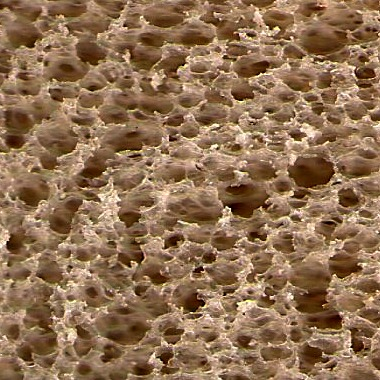
\includegraphics[scale=1.3]{imagenes/lactal31}}}$
$\vcenter{\hbox{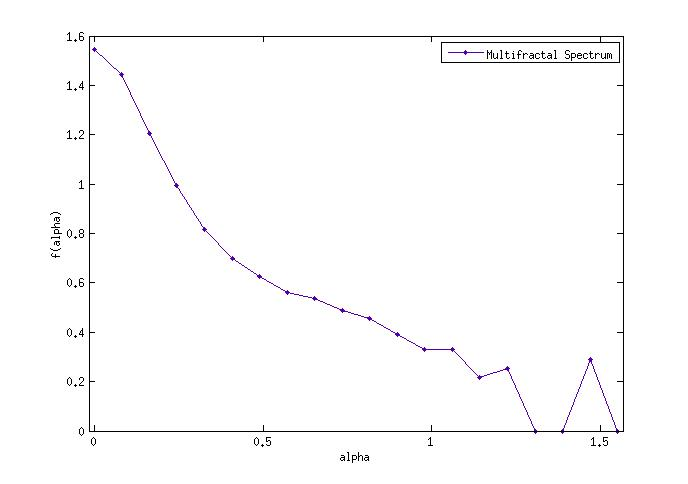
\includegraphics[scale = 0.4]{imagenes/emf}}}$
\caption{Bread image and its corresponding multifractal spectrum (20 FDs)}
\label{fig:emf}
\end{figure*}


\subsection{Sandbox Method}
This method was introduced in \cite{Tel89} and it is useful to obtain generalized multifractal dimensions. These dimensions are linked to the singularity multifractal spectrum via a Legendre Transform:

\begin{equation}
D(q) = q h(q) - F(h),
\label{eqn:eqnLeg1}
\end{equation}

\begin{equation}
h(q) \cong \alpha(q) = \mathrm{d}(D(q))/\mathrm{d}q,
\label{eqn:eqnLeg2}
\end{equation}
where $\alpha$ is an approximation of the H\"older exponent $h$.

We first need to binarise the image, and then, $N$ points belonging to the structure ({\em i.e.}, regions with white pixels) should be randomly selected, counting for each point the number of white pixels inside a box of diameter $R$, centred at the point. The generalized sandbox dimension of order $q$ is obtained as \cite{Bert94}

\begin{equation}
D_{q} = \lim_{R\rightarrow0}{\frac{1}{q-1} \frac{\log \bigg \lbrack\frac{1}{N}\displaystyle \sum_{i=1}^{N}{p_{i}^{q-1}}\bigg \rbrack}{\log R}},
\label{eqn:eqn1}
\end{equation}

where $p_{i}$ is the number of points in the box of radius $R$ centred at the point $i$. An average is made over the $N$ points. Equation (\ref{eqn:eqn1}) can also be stated as

\begin{equation}
D_{q} = \lim_{R\rightarrow0}{D_{q}(R)}.
\end{equation}

In practice we perform a linear fit between the values of $D_{q}(R)$ and $R$ for $R$ in $[R_{min}, R_{max}]$. The latter value will be determined based on the accuracy of the application that we need.


\section{Applications}

\subsection{Image Clasification}
For each material, the results obtained in the classification process are useful in quality measurements of real samples and also in the validation of synthetic representations of them. In other words, the classification is useful to determine if a given image presents the observed features in that material, allowing to associate quality measure parameters to the material.

It is possible to use the obtained dimensions as image features. As an example, we will describe how different bread crumbs could be automatically classified based on these features.

\subsubsection{Bread Crumb Classification}
Twenty images of four different bread types ({\em lactal}, {\em baguette}, {\em salvado} and {\em sandwich}), counting $80$ images, were obtained using an electric slicer. The images were digitalised using an HP PSC 1210 scanner and they were saved in TIFF format. Images showed a resolution of $380 \times 380$ pixels (the maximum possible area for the four bread types) and $350$ dpi ($1$ pixel $= 0.00527 mm^{2}$). Then the images were converted to grey scale ($8$ bits). In addition, $20$ images of each bread type were acquired with a digital camera, using the same spatial resolution, counting $80$ images. The illumination conditions of these images were different from that of the scanner in order to test for the robustness of the method. In Fig.~\ref{fig:camera} four examples of bread images from the camera are shown. We also employed one hundred randomly selected images from the CalTech101~\cite{FeiFei04} dataset in order to test the method's performance with non-bread images. In Fig.~\ref{fig:nonbread} four examples of non-bread images from this dataset are shown. 

\begin{figure*}[htb]
\centering
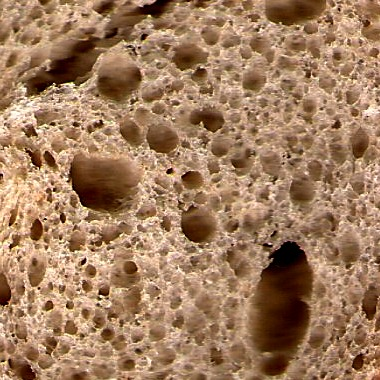
\includegraphics[scale=1]{imagenes/baguette20}
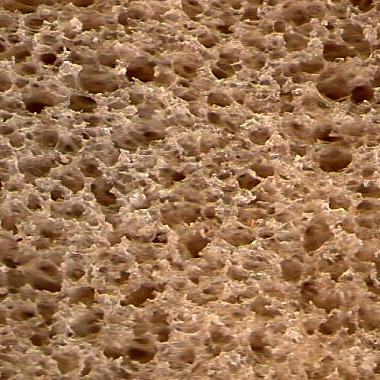
\includegraphics[scale=1]{imagenes/lactal14}
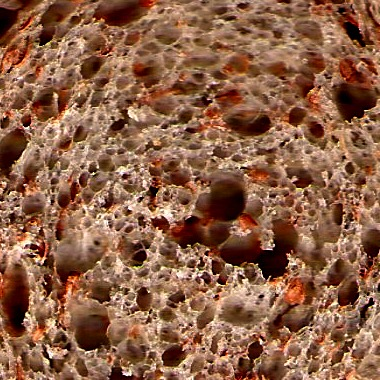
\includegraphics[scale=1]{imagenes/salvado43}
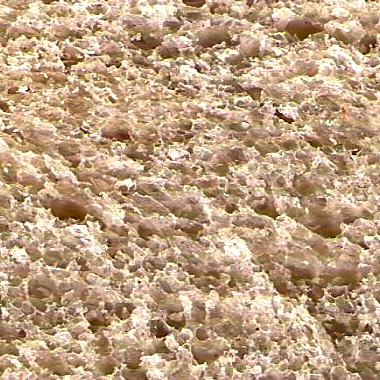
\includegraphics[scale=1]{imagenes/sandwich43}
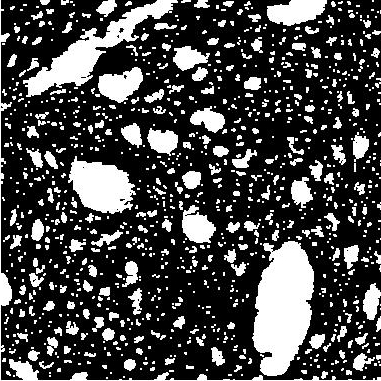
\includegraphics[scale=0.205]{imagenes/baguette20bin}
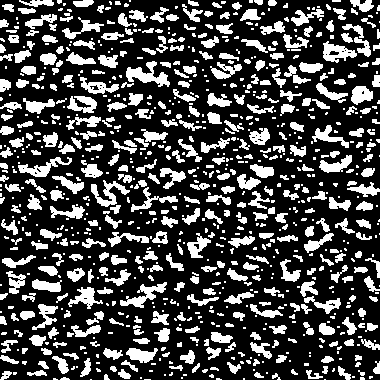
\includegraphics[scale=0.26]{imagenes/lactal14bin}
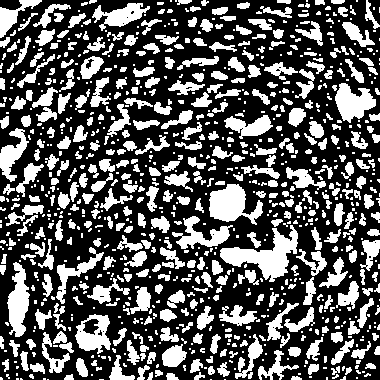
\includegraphics[scale=0.26]{imagenes/salvado43bin}
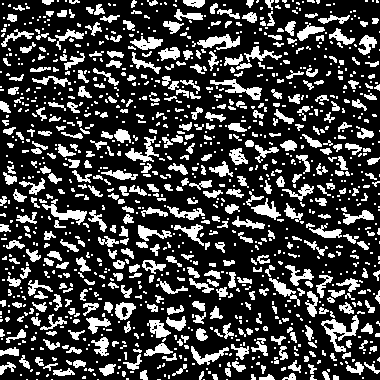
\includegraphics[scale=0.26]{imagenes/sandwich43bin}
\caption{Digitalised images of {\em baguette}, {\em lactal}, {\em salvado} and {\em sandwich} bread types from a scanner with its binarisations}
\label{fig:bread}
\end{figure*}

\begin{figure*}[htb]
\centering
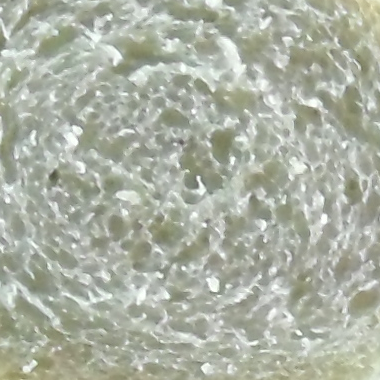
\includegraphics[scale=0.20]{imagenes/b}
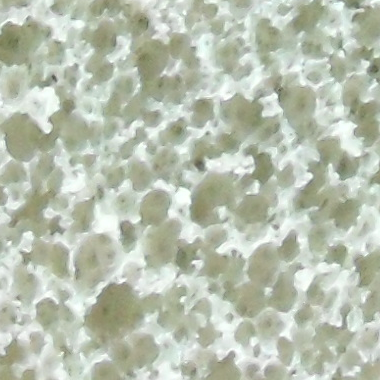
\includegraphics[scale=0.20]{imagenes/l19}
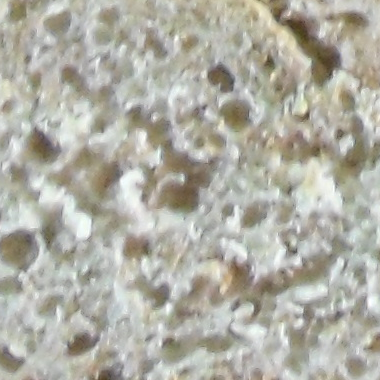
\includegraphics[scale=0.20]{imagenes/s7}
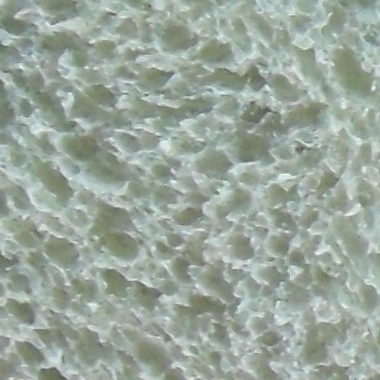
\includegraphics[scale=0.20]{imagenes/Sa14}
\caption{Digitalised images from a digital camera}
\label{fig:camera}
\end{figure*}

\begin{figure*}[htb]
\centering
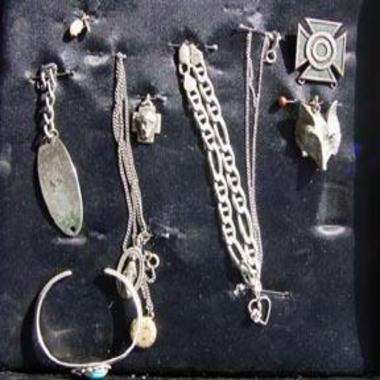
\includegraphics[scale=0.20]{imagenes/image_0036}
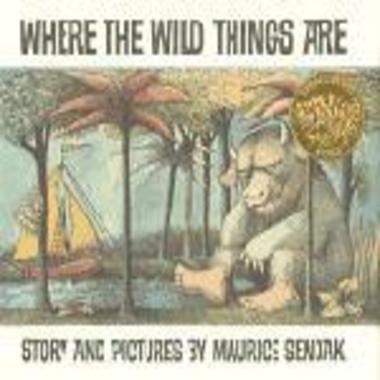
\includegraphics[scale=0.20]{imagenes/image_0041}
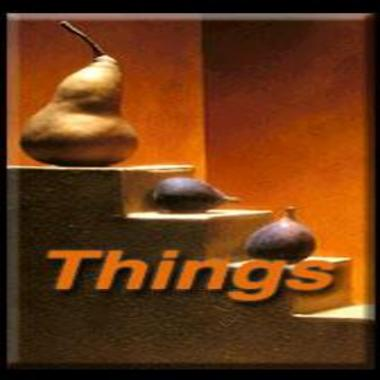
\includegraphics[scale=0.20]{imagenes/image_0042}
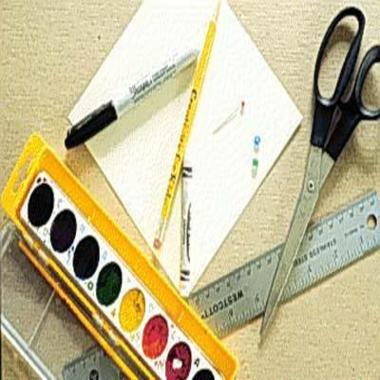
\includegraphics[scale=0.20]{imagenes/image_0048}
\caption{Images from the dataset CalTech101}
\label{fig:nonbread}
\end{figure*}

For the binarisation of the images, the algorithm presented in \cite{White83} was used. This algorithm applies a local thresholding schema, which showed better results than using a global thresholding schema. Particularly, the algorithm presented in \cite{Huang95} and used in \cite{Gonzales2008}, showed poor results when the illumination conditions vary. In Fig.~\ref{fig:bread} an image of each bread type used in this work (top row) and its resulting binarisation using the proposed algorithm (bottom row) is shown.  

\subsubsection{Results}

{\em Support Vector Machines} (SVM)~\cite{Boser92} were used to perform the classification, using the {\em libsvm}~\cite{Chang2011} implementation. The method of {\em k-fold cross validation} was employed in order to validate the results with $k = 4$, {\em i.e.}, $75\%$ of samples are used as training and $25\%$ as testing (then switching the training and testing samples). The cross validation is applied only to scanner samples.

A robust bread crumb classifier could be used to make the classification process independent of the image capturing condition. In each case, we performed a test in order to show the accuracy of the classifiers when there is a capturing condition mismatch between training and testing samples, {\em i.e.}, when training with scanner samples and testing with camera samples. Based on the randomness in the method's point selection, we made an {\em ensemble} of $10$ trained SVMs models, in which each SVM prediction {\em votes} for one bread type. Then the most appearing class (the most voted class for each image) is selected in each case. In the case of cross validation, we made an average of the percentages obtained. Table \ref{table:tableFirstTest} shows classification results when varying different parameters of the method.

\begin{table}[htb]
\centering
\begin{tabular}{|c|c|c|c|c|c|}
    \hline
    \# Fractal Dimensions & $14$ & $8$ & $20$ & $20$ & $30$\\
    \hline
    $R_{max}$ & $40$ & $20$ & $20$ & $20$ & $20$\\
    \hline
    \# Points & $900$ & $900$ & $900$ & $2500$ & $900$\\
    \hline
    Cross Validation  & $75,5\%$ & $76,2\%$ & $77,1\%$ & $79,8\%$ & $77,4\%$\\
    \hline
    Robustness & $46\%$ & $44\%$ & $49\%$ & $49\%$ & $47\%$ \\
    \hline
\end{tabular}
\caption{Results obtained with different parameters}
\label{table:tableFirstTest}
\end{table}


In Table \ref{table:ConfusionMatrixFractal} the confusion matrix of the data using the classifier in the robustness test is shown. The matrix shows that the classifier tends to label most of the data to the non-bread class. It also shows that the {\em baguette} bread type is successfully discriminated.
\begin{table}[htb]
\centering
\begin{tabular}{|c|c|c|c|c|c|}
    \hline
    Classes & {\em baguette} & {\em lactal} & {\em salvado} & {\em sandwich} & non bread\\
    \hline
    \hline
    {\em baguette}  & $20$ & $0$ & $0$ & $0$  & $0$\\
    \hline
    {\em lactal}    & $1$ & $1$ & $0$ & $0$  & $18$\\
    \hline
    {\em salvado}   & $0$ & $3$ & $2$ & $0$  & $15$\\
    \hline
    {\em sandwich}  & $0$ & $4$  & $0$ & $0$ & $16$\\
    \hline
    non bread       & $1$ & $0$  & $0$ & $0$  & $19$\\
    \hline
\end{tabular}
\caption{Confusion Matrix for the multifractal features}
\label{table:ConfusionMatrixFractal}
\end{table}

It can be seen that the values for the cross validation and for the robustness tests are similar when varying the parameters of the method.

\subsection{Image enhancement}
\subsection{Esge Detection}
\subsection{Medical Applications}




\bibliography{bibliografia/bib}
\bibliographystyle{unsrt}
\end{document}
